\chapter{Introduction}

Predicting the behaviour of complex systems has always been an important goal of scientific research. From predicting the motion of stars and planets in our solar system, to understanding the behaviour of complex systems showing chaotic behaviours. In history, before scientists were able to find analytical solutions to many problems, they often relied on simulations. A
celebrated example are the astronomical clocks that
were built in Asia and Europe in the period between 1000 and
1500, such as the famous astronomical clock in Prague (1410) or the Zytglogge in Bern (1530). They were used to predict the position of the planets and the constellations, the phases of the moon and its eclipses \cite{bloch2012}.

With the advent of quantum mechanics, a new kind of problems for which no analytical solution is possible was found. Given the high dimensionality of the Hilbert space, classical computers cannot be used to find numerical solutions to quantum many body problems. For example, simulating a system of $N=36$ qubit using two double-precision floating-point numbers to store a complex number, would require approximately $2^{N+1} \cross 8$ byte $=$ 1 Terabyte of memory. For every additional qubit, this number would double.

Richard Feynman was the first to propose to use a quantum system to handle this complexity making use of the law of quantum mechanics itself. In 1982, he proposed to make use of "one controllable quantum system simulate another" \cite{feynman1982}. In this way, a system of $N$ quantum particles could be simulated using another system of $N$ qubits. The problem is then moved to finding a system that can be easily tuned and controlled, such that it can be used to simulate a wide range of problems.

\section{Analog and digital quantum simulation}

Two different approaches have arisen in the past years: (digital) quantum computation and (analog) quantum simulation. In the first case, the information is encoded in qubits that can be in two computational states $\ket{0}$ and $\ket{1}$. Among the most promising platforms that have been proposed to realize such a quantum computer, we cite the use of superconducting circuits \cite{blais2021a}, Rydberg atoms \cite{wu2021a} and trapped ions \cite{bruzewicz2019}. The latter approach requires a direct mapping of the original problem (i.e. its Hamiltonian) to the simulating system. For this goal, the use of ultracold quantum gases has become increasingly popular \cite{bloch2012}.

For example, a system of electrons moving in an ionic periodic lattice potential, can be simulated using a gas of fermionic atoms trapped in an optical lattice potential. Here, the periodic potential
through which the particles move is generated externally by making
use of the interference pattern of overlapping laser beams \cite{bloch2008}. It is performing an experiment of this kind that Bloch oscillations, predicted by Felix Bloch \cite{bloch1929a} in 1929, were directly observed in a cloud of ultracold cesium atoms \cite{dahan1996} in 1996, after being observed through the emission of THz radiation by the electrons in a semiconductor super lattice by Feldman and Leo \cite{feldmann1992} in 1992.

In the following years, new interesting experiments were proposed to simulate the behaviour of different quantum systems. Among them, we cite the use of optical lattices to investigate insulating and superfluid quantum phases \cite{greiner2002}, the use of cavities to mediate long range interactions \cite{landig2016} and the observation of quantized conductance in neutral matter \cite{krinner2015}. I will focus on this last experiment, since my project was related to it.

\section{Transport experiments}
Transport experiments study the transport properties of particles moving from one reservoir to another. Krinner \emph{et al.} reported the observation of quantized conductance in the transport of neutral atoms driven by a chemical potential bias \cite{krinner2015}. Their experiment let them investigate
quantum conductors with wide control not only over the channel
geometry, but also over the reservoir properties, such as interaction strength, size and thermalization rate.

\begin{figure}
    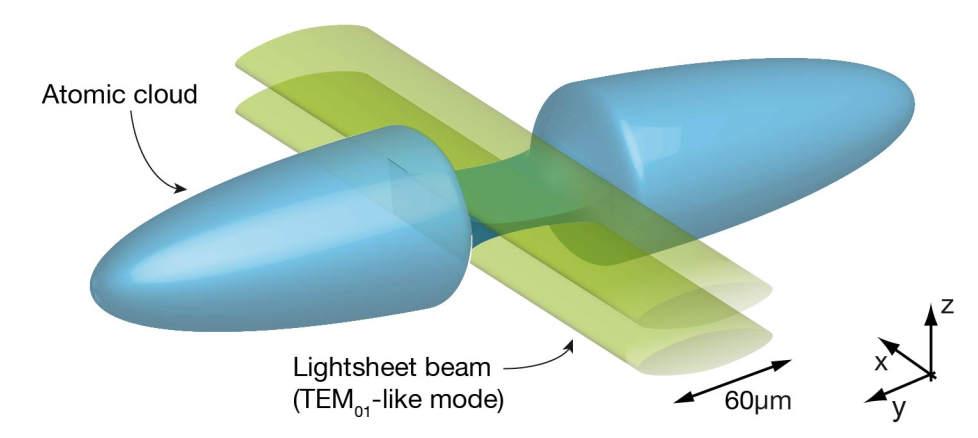
\includegraphics[width=\textwidth]{figures/reservoir.png}
    \caption{Experimental setup. A cloud of atoms is trapped in a cigar-shaped potential. A blue-detuned $\text{TEM}_{01}$ laser mode propagating in the $x$ direction defined a quasi-2D channel connecting two smoothly connected reservoirs. Figure from Krinner \cite{krinner2015}.}
    \label{fig:lithium_apparatus}
\end{figure}

The basic setup of the experiment is shown in \cref{fig:lithium_apparatus}. A cloud of atoms is radially trapped with a dipole trap realized with a red-detuned laser. Along the $y$ axis the confinement is produced by the magnetic field curvature of the Feshbach coils. This defines a cigar-shaped cloud elongated in the $y$ direction. The cloud is then split in two reservoir connected by a quasi-2D channel sending a blue-detuned $\text{TEM}_{01}$ laser mode in the $x$ direction. The blue-detuned laser creates a repulsive potential that confines the atoms in a quasi-2D region. The experiment is then carried on creating a chemical potential imbalance between the two reservoir and studying the conduction of atoms between them. Different experiments can be realized creating a temperature imbalance or a spin imbalance between the reservoirs.

The focus of this thesis is on red-detuned laser generating the 2D channel. In the current experiment, the laser is in a $\text{TEM}_{01}$ mode. The beam is shaped through a series of optical components shown in \cref{fig:beam_shaper}. It is clear that the potential inside the channel region is not uniform along the $y$ direction. The conductance is influenced by this varying potential and it would be desirable to have a uniform region connecting the two reservoir.

\begin{figure}
    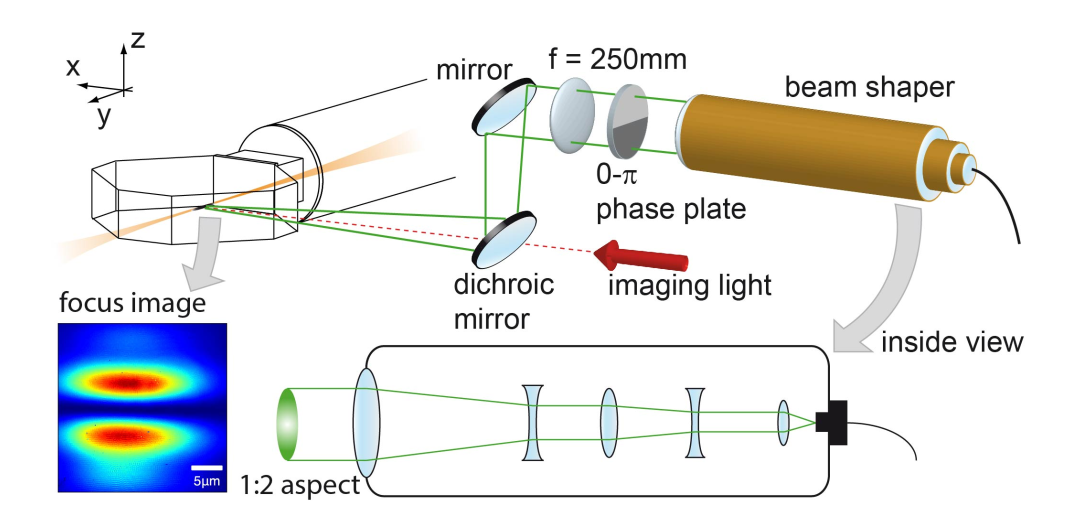
\includegraphics[width=\textwidth]{figures/beam_shaper.png}
    \caption[short]{Generation of the $\text{TEM}_{01}$ mode for the creation of 2D channel. A set of spherical and cylindrical lenses is used to expand the beam in the $z$ direction. The beam is then sent to a $0-\pi$ phase plate and focused through a \SI{250}{mm} lens on the atomic cloud. Figure from Krinner \cite{krinner2015}.}
    \label{fig:beam_shaper}
\end{figure}

The opportunity to create such a uniform 2D channel was previously investigated by Moritz Schmidt in his semester project \cite{schmidt2021}. Schmidt considered two options for generating a uniform light sheet: the use of liquid-crystal spatial light modulators and of custom-made glass $0-\pi$, top-hat phase-plates. It was found that this second option is more suitable to the experiment, being able to reach the experimental requirements, and at the same time considerably cheaper.

\section{Outline}
In this report, I analyse and characterize the custom-made phase plate ordered for the creation of the uniform light sheet. I will start by reviewing the theory behind spatial light modulation, focusing on how a phase plate can be used to shape light beams. Then I will present the apparatus